\documentclass[12pt]{article}
\usepackage[papersize={8cm,12cm},margin={.5cm,.5cm}]{geometry}
\usepackage{common}
\usepackage{amssymb}
\begin{document}
\begin{problem}
\item[8.] 圖(八)中,$I$ 點為 $\triangle{ABC}$ 的內心,$D$ 點在 $\overline{BC}$ 上,且 $\overline{ID} \perp \overline{BC}$。若 $\angle{B} = 44^\circ$,$\angle{C} = 56^\circ$,則 $\angle{AID}$ 的度數為何?
  \begin{figure}[ht]
    \centering
    \vspace*{-1ex}
    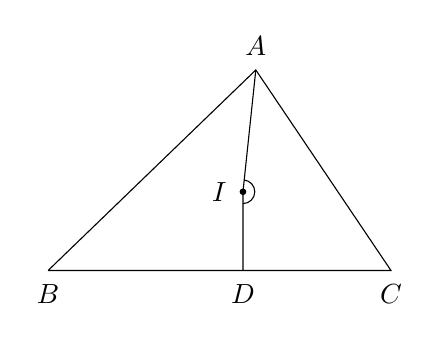
\begin{tikzpicture}
      \filldraw (0,0) circle (1pt);
      \draw (0,-.15) arc (-90:84:.15);
      \draw (0,-1) -- (0,0) -- (.163,1.547);
      \draw (-2.475,-1) -- (1.88,-1) -- (.163,1.547) -- (-2.475,-1);
      \node at (.163,1.847) {$A$};
      \node at (-2.475,-1.3) {$B$};
      \node at (1.88,-1.3) {$C$};
      \node at (0,-1.3) {$D$};
      \node at (-.3,0) {$I$};
    \end{tikzpicture}
    \vspace*{-1ex}
    \caption*{圖(八)}
    \vspace*{-2ex}
  \end{figure}
  \begin{choices}
    \item 174
    \item 176
    \item 178
    \item 180
  \end{choices}
\end{problem}
\end{document}
